\section{Statistic Analysis}\label{statistic}
In this section, we will discuss some statistic analysis results of UFO dataset. Figure \ref{map} and \ref{heat} demonstrate the cumulative sighting numbers from 1950 to 2016 across U.S. The UFO sightings distributed across U.S. unevenly --- California reports more UFO sightings than the other states. We believe this is because of its unique geographical conditions --- on the coast and with desert. Having the same geographical conditions, Texas, Florida and Washington also report more sightings than other states. Another kind of geographical condition, near the Great Lakes, also results in more sighting numbers, for example in Illinois, Michigan, Ohio, Pennsylvania and New York. As shown in figure \ref{mean}, we calculate estimated marginal means of duration of UFO sightings for each state. Just like what we expected, California also has an extremely high mean value than other states. 

\begin{figure}[H]
\centering 
\subfigure[state distribution]{\label{map}
\begin{minipage}[b]{0.5\textwidth}
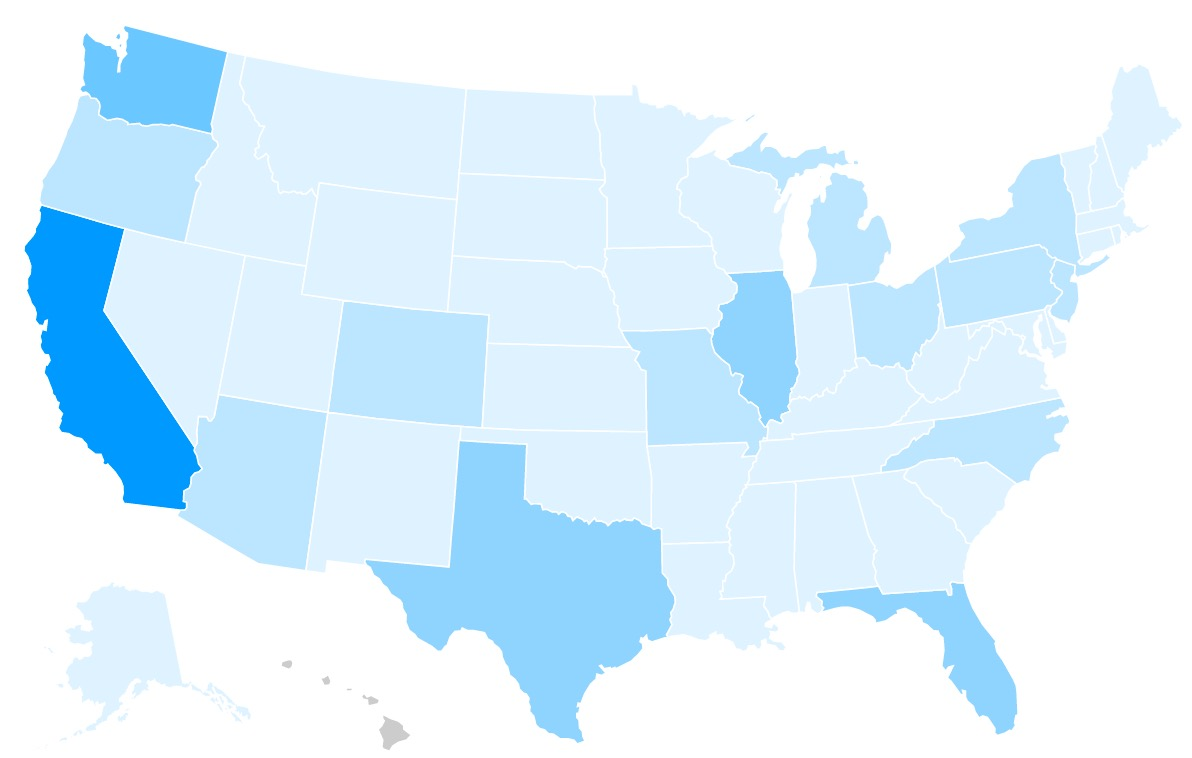
\includegraphics[width=1\textwidth]{figure/sighting_number.jpg}
\end{minipage}
}
\subfigure[heat map]{\label{heat}
\begin{minipage}[b]{0.43\textwidth}
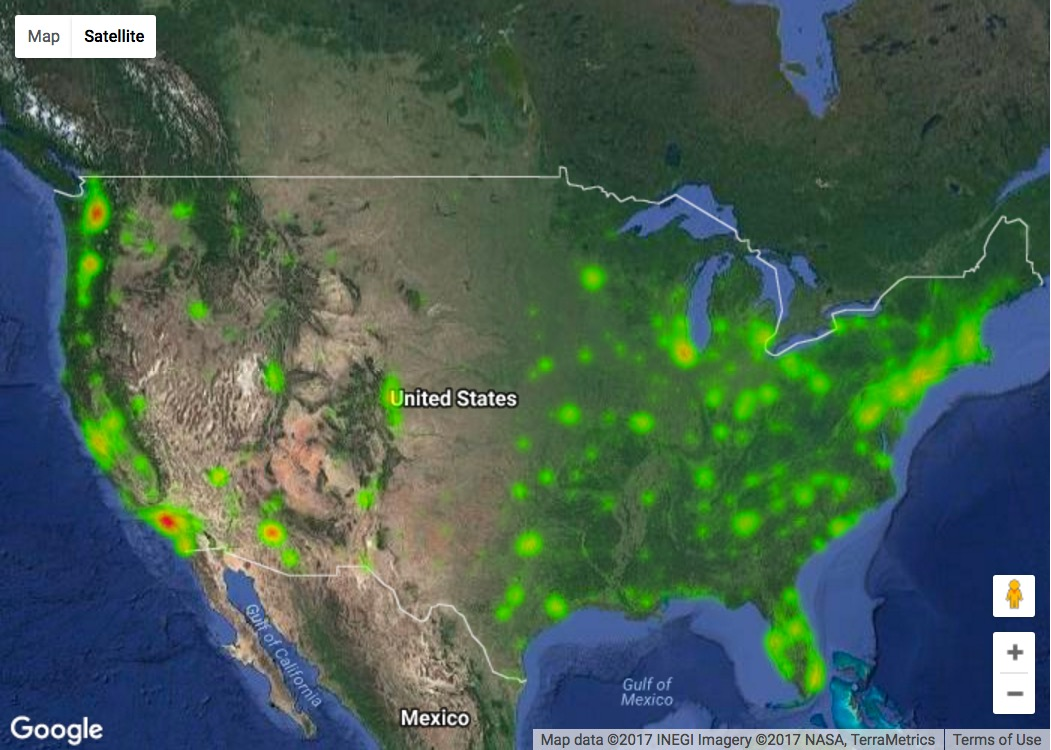
\includegraphics[width=1\textwidth]{figure/heat_map.jpg}
\end{minipage}
}
\caption{cumulative distribution around U.S.}
\end{figure}


\begin{figure}[H]
    \centering
    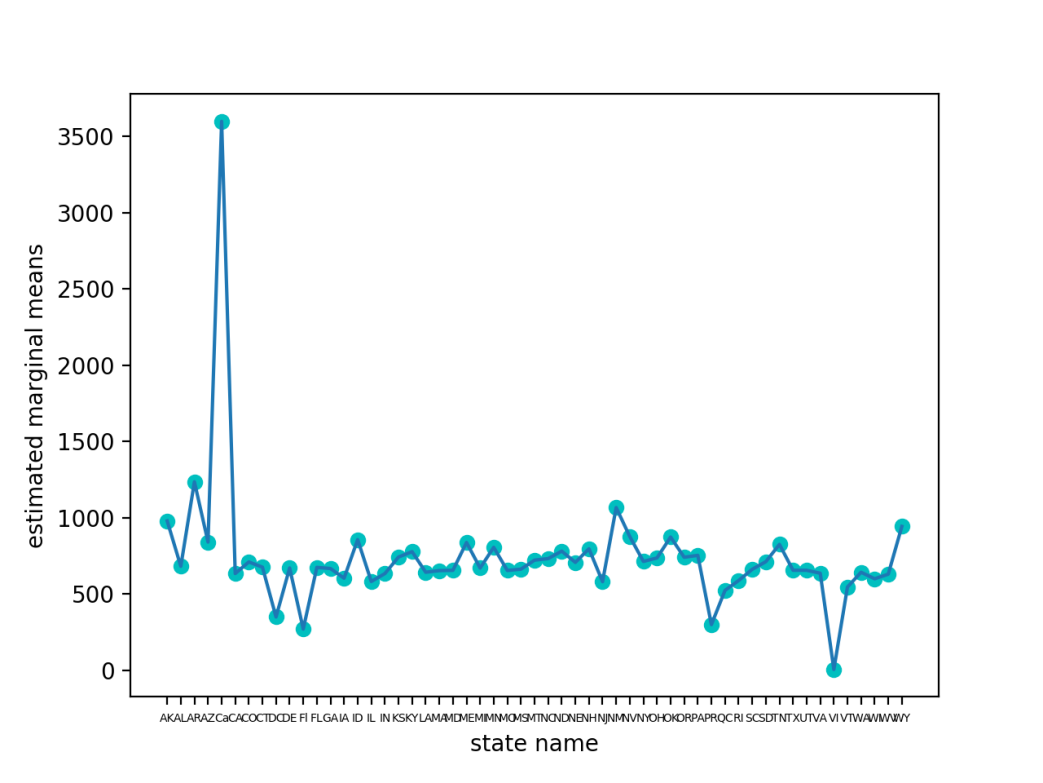
\includegraphics[width=10cm]{figure/marginal.png}
    \caption{estimated marginal means of duration for each state}
    \label{mean}
\end{figure}

Next, we analyze relations among different fields of UFO sighting reports themselves. Pie chart \ref{shape} shows that many UFO looks like light (21\%), circle (10\%) and triangle (10\%), with about 10\% witnesses are not sure about shapes. 

\begin{figure}[H]
    \centering
    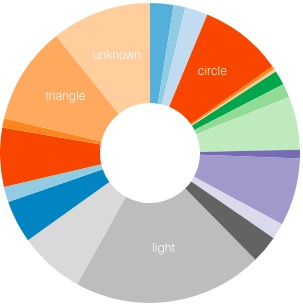
\includegraphics[width=6.5cm]{figure/shape.jpg}
    \caption{shape distribution}
    \label{shape}
\end{figure}

\begin{figure}[H]
\centering 
\subfigure[weather]{\label{weather}
\begin{minipage}[b]{0.3\textwidth}
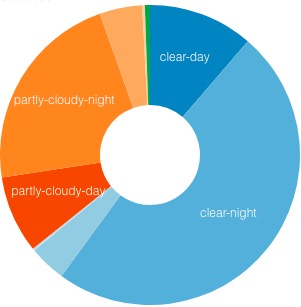
\includegraphics[width=1\textwidth]{figure/weather.jpg}
\end{minipage}
}
\subfigure[hour]{\label{hour}
\begin{minipage}[b]{0.55\textwidth}
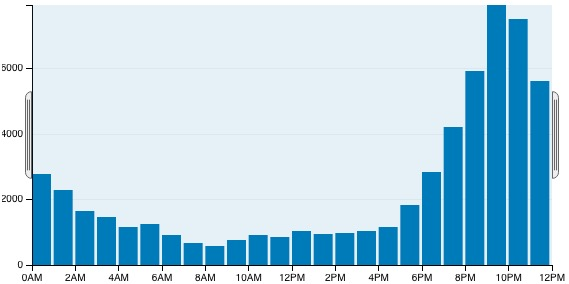
\includegraphics[width=1\textwidth]{figure/hour.jpg}
\end{minipage}
}
\subfigure[weekday]{\label{weekday}
\begin{minipage}[b]{0.55\textwidth}
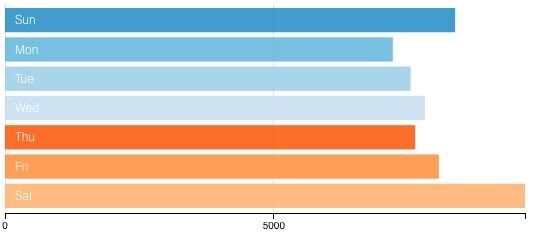
\includegraphics[width=1\textwidth]{figure/weekday.jpg}
\end{minipage}
}
\caption{weather and time distribution}
\end{figure}

For one thing, most UFO sightings occurred at night, regardless of how the weather is (as shown in figure \ref{weather}), which is consistent with figure \ref{hour} where most sightings occurred between 8 PM and 12 PM during a day. This observation reflects a basic rule about when  UFO appears --- mostly at night. For another thing, the numbers of sightings on weekends are slightly larger than those on weekdays. However, we do not accept this observation as a rule for UFO sightings. Such phenomenon happens probably because most people are busy at work on work days and they go back home early at night for rest, while they attend outdoor activities during weekend nights. Given that UFO tends to appear during the night, people have less chance to sight one during weekdays.




